\subsection{Multinomial Logistic Regression}

\subsubsection{Mô hình cho tập dữ liệu chỉ bao gồm các quan sát có cột "emailtotal" không phải giá trị null}

\begin{enumerate}[label=(\alph*)]
    \item Đầu vào mô hình là vector thu được từ phân tích thành phần chính sử dụng thuật toán PCA
    
    Ta có bảng kết quả huấn luyện mô hình:

    \begin{python}
        precision    recall  f1-score   support

        Keeping house       0.00      0.00      0.00        58
                Other       0.00      0.00      0.00         8
              Retired       0.00      0.00      0.00       109
               School       0.00      0.00      0.00        14
     Temp not working       0.00      0.00      0.00        15
     Unempl, laid off       0.00      0.00      0.00        25
     Working fulltime       0.53      1.00      0.69       351
     Working parttime       0.00      0.00      0.00        80
     
             accuracy                           0.53       660
            macro avg       0.07      0.12      0.09       660
         weighted avg       0.28      0.53      0.37       660
    \end{python}

    và ma trận nhầm lẫn:

    \begin{figure}[H]
        \centering
        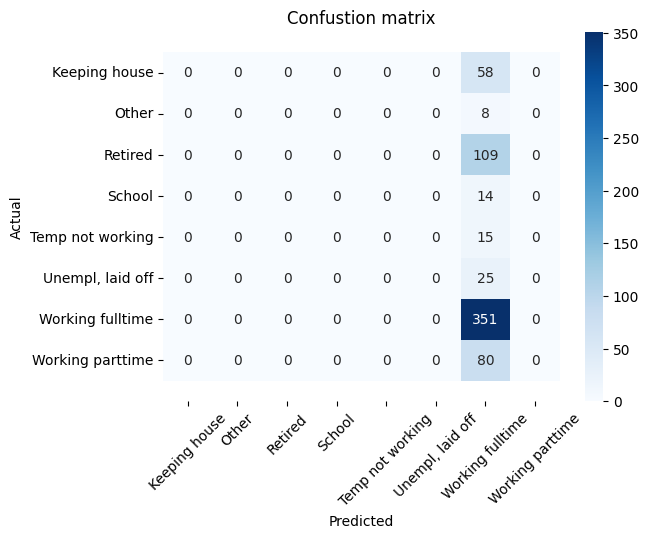
\includegraphics[width=0.6\textwidth]{figures/Thanh/Models/Logistic/Non_null_models_confusion_matrix_Logistic_PCA_features.png}
        \caption{Ma trận nhầm lẫn của mô hình Multinomial Logistic Regression khi vector đầu vào được phân tích thành phần chính}
        \label{fig:Non_null_models_confusion_matrix_Logistic_PCA_features}
    \end{figure}

    Ta nhận thấy kết quả phân loại không tốt, trừ nhóm làm việc toàn thời gian có độ hồi tưởng là 1 và độ chính xác là 0.53 thì tất cả độ chính xác và độ hồi tưởng của các lớp khác đều bằng 0.
    Nhìn vào ma trận nhầm lẫn ở hình \ref{fig:Non_null_models_confusion_matrix_Logistic_PCA_features} ta nhận thấy mô hình dự đoán tất cả các quan sát vào lớp làm việc toàn thời gian.
    Lý do là vì từ phần phân tích dữ liệu, ta thấy phân phối của các thành phần chính tương ứng với các nhóm trong cột wrkstat gần như cùng hình dạng, trộn lẫn vào nhau.
    Mô hình sẽ khó phân biệt được quan sát nào thuộc lớp nào.
    Trong quá trình học, mô hình biết số quan sát thuộc lớp làm việc toàn thời gian có số lượng nhiều nhất.
    Hàm mục tiêu của mô hình là hàm cross entropy.
    Vì do phân phối của các lớp gần giống nhau hoàn toàn, mô hình sẽ học bằng cách là dự đoán các tất cả các quan sát đến vào cùng một lớp.
    Khi dự đoán như vậy để hàm cross entropy trên dữ liệu là nhỏ nhất, mô hình buộc phải chọn dự đoán tất cả các quan sát có số lượng nhiều nhất mà mô hình đã biết từ tập huấn luyện.

    Ta sẽ phân tích ngược trở lại trọng số của các tham số tương ứng với các đặc trưng của vector ban đầu từ các tham số ứng với các đặc trưng của các thành phần chính:

    \begin{figure}[H]
        \centering
        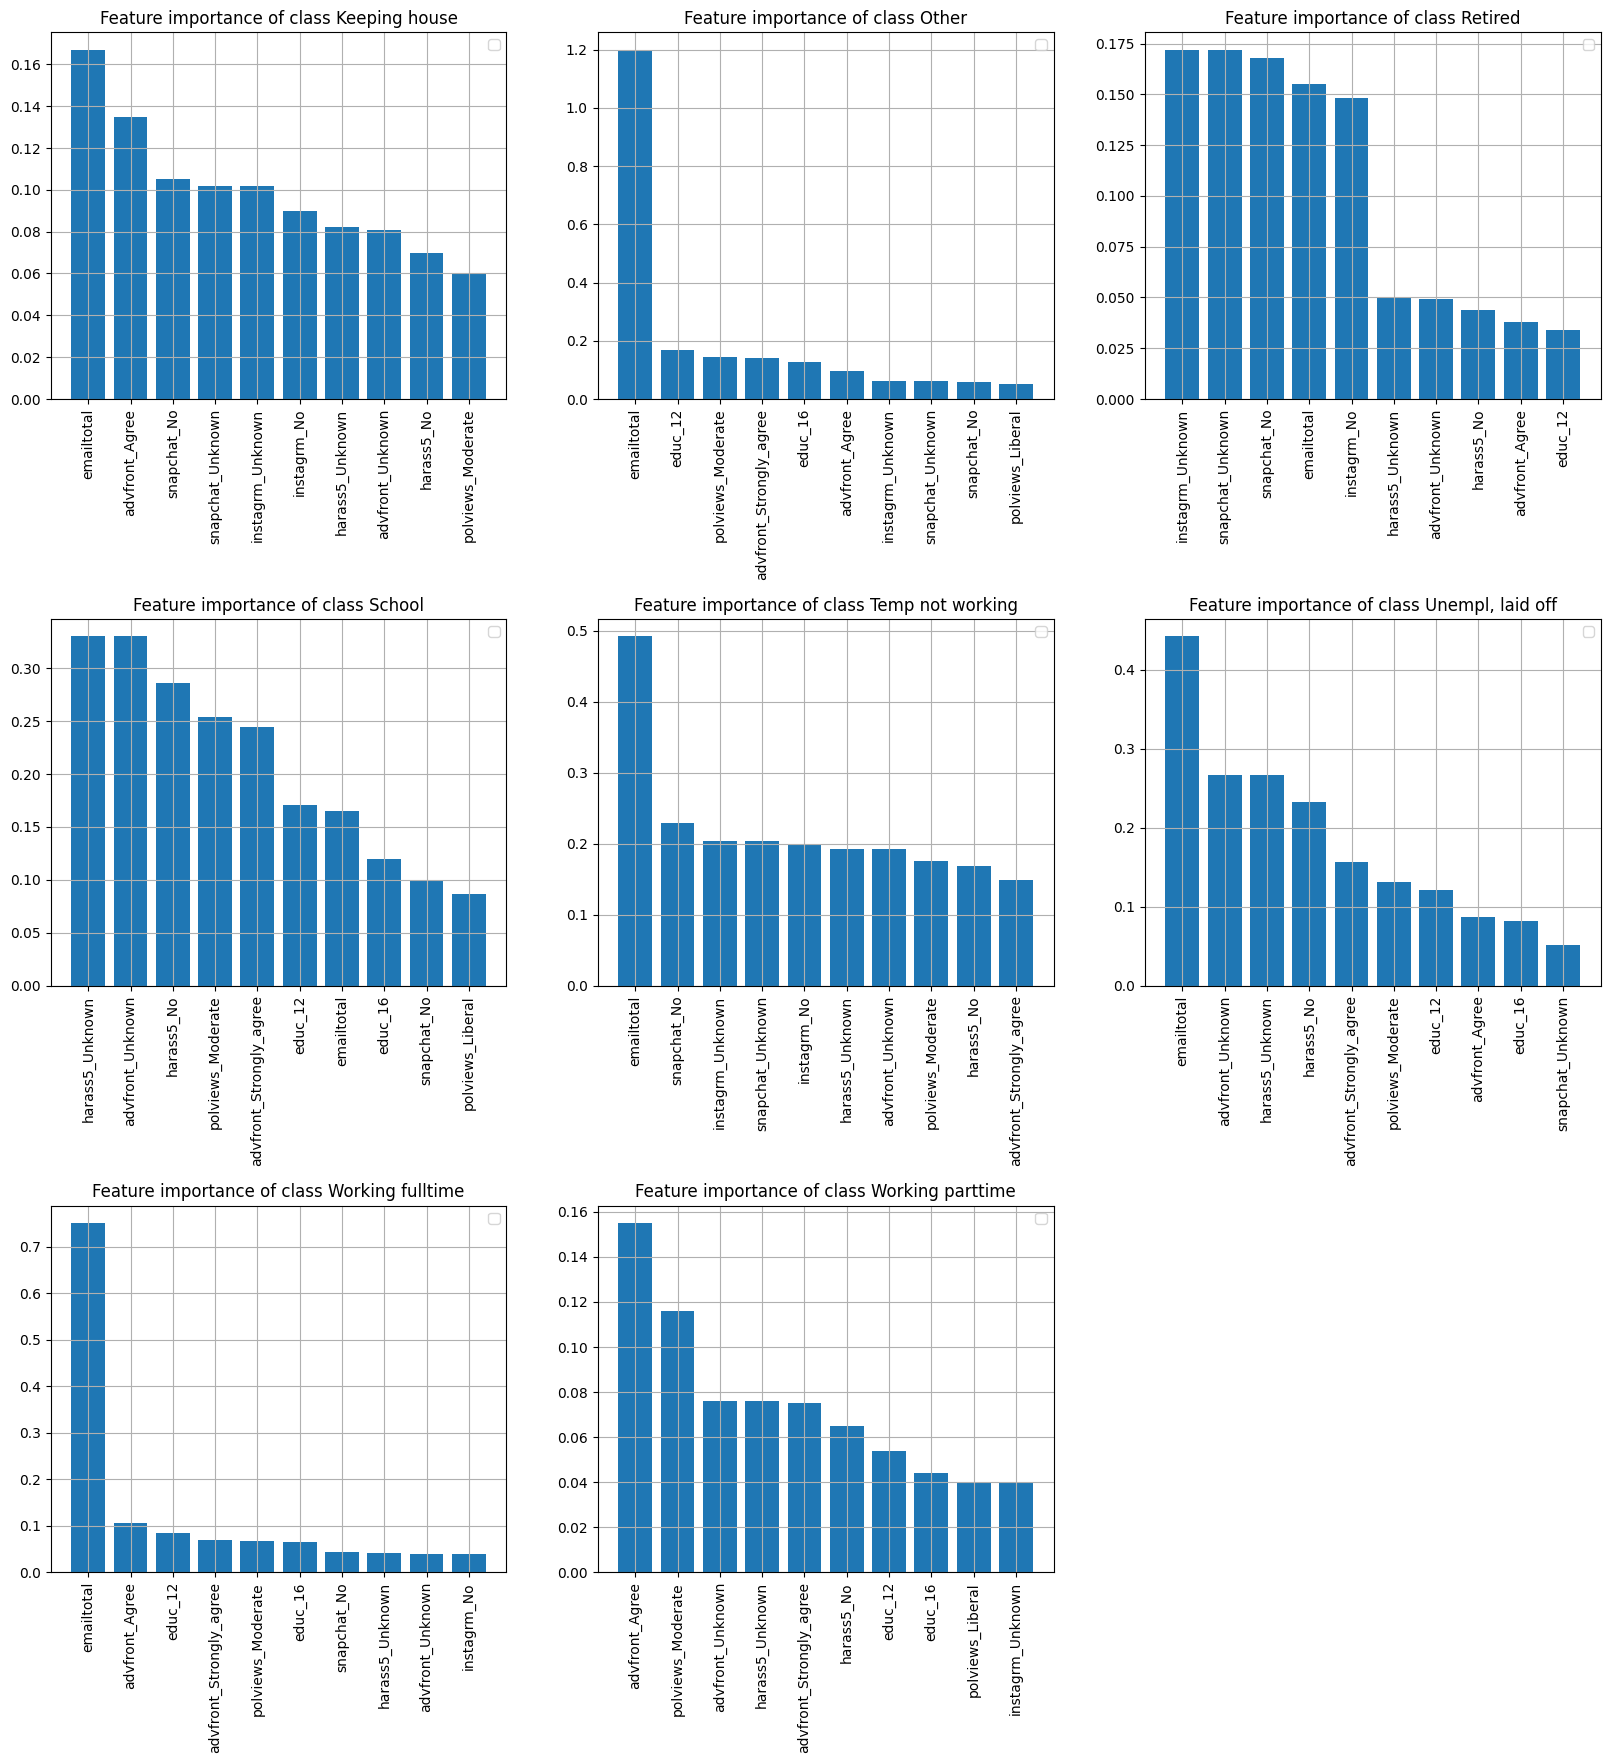
\includegraphics[width=0.6\textwidth]{figures/Thanh/Models/Logistic/Non_null_models_Feature_Importance_Logistic_PCA_features.png}
        \caption{Biểu đồ cột sắp xếp độ lớn giảm dần (trị tuyệt đối) tham số của các đặc trưng ứng với từng nhãn}
        \label{fig:Non_null_models_Feature_Importance_Logistic_PCA_features}
    \end{figure}

    Ta có biểu đồ cột sắp xếp độ lớn giảm dần (trị tuyệt đối) tham số của các đặc trưng ứng với từng nhãn giả thể hiện ở hình \ref{fig:Non_null_models_Feature_Importance_Logistic_PCA_features}.
    Ta nhận thấy các cột có trọng số lớn và ảnh hưởng nhiều tới các các nhãn đầu ra là emailtotal, snapchat\_Unknown và instagrm\_Unknown.
    Hai đặc trưng snapchat\_Unknown và instagrm\_Unknown có tần suất xuất hiện lớn trong tập dữ liệu.
    emailtotal ảnh hưởng khá nhiều đến việc phân chia dữ liệu do những người làm việc toàn thời gian có thời gian dành cho email có xu hướng lớn hơn các nhóm hình thức làm việc còn lại.

    \begin{figure}[H]
        \centering
        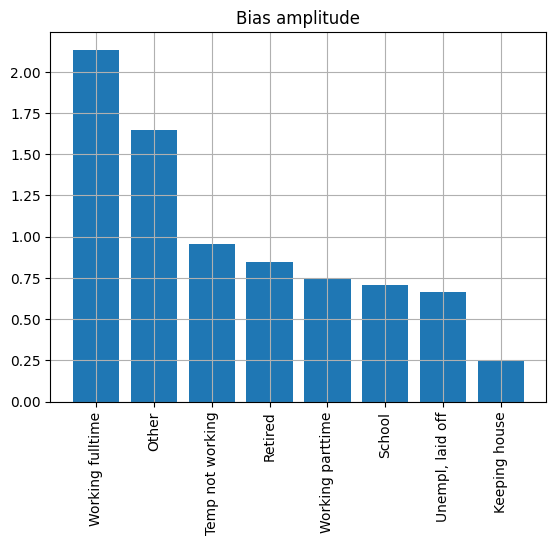
\includegraphics[width=0.6\textwidth]{figures/Thanh/Models/Logistic/Non_null_models_Bias_Importance_Logistic_PCA_features.png}
        \caption{Biểu đồ cột thể hiện độ lớn của các bias tương ứng với từng nhãn}
        \label{fig:Non_null_models_Bias_Importance_Logistic_PCA_features.png}
    \end{figure}

    Hình \ref{fig:Non_null_models_Bias_Importance_Logistic_PCA_features.png} thể hiện độ lớn của các bias tương ứng với từng nhãn giả.
    Bias tương ứng với lớp làm việc toàn thời gian cao nhất.
    Điều này cũng khá dễ hiểu khi mô hình luôn muốn kết quả đầu ra tương ứng với lớp làm việc toàn gian cao nhất khi mô hình có xu hướng phân loại mọi quan sát vào lớp làm việc toàn thời gian.

    \item Vector đầu vào là vector gốc ban đầu
    
    Ta có bảng kết quả huấn luyện mô hình:

    \begin{python}
        precision    recall  f1-score   support

   Keeping house       0.21      0.09      0.12        58
           Other       0.00      0.00      0.00         8
         Retired       0.36      0.14      0.20       109
          School       0.00      0.00      0.00        14
Temp not working       0.00      0.00      0.00        15
Unempl, laid off       0.00      0.00      0.00        25
Working fulltime       0.56      0.90      0.69       351
Working parttime       0.19      0.06      0.09        80

        accuracy                           0.52       660
       macro avg       0.16      0.15      0.14       660
    weighted avg       0.40      0.52      0.42       660
    \end{python}

    và ma trận nhầm lẫn:

    \begin{figure}[H]
        \centering
        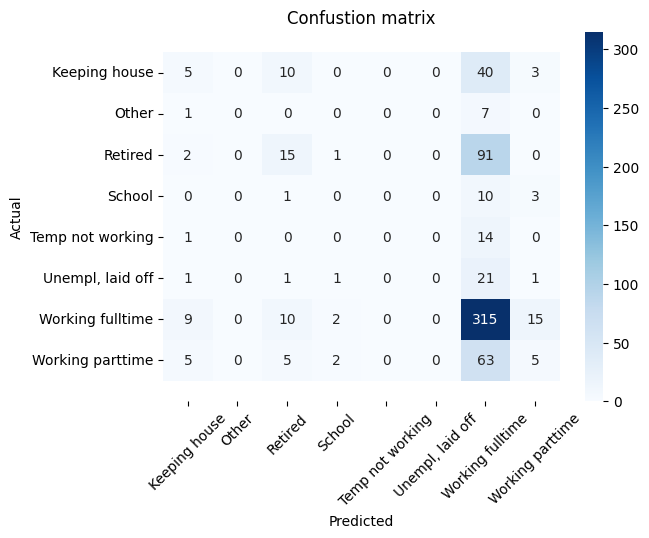
\includegraphics[width=0.6\textwidth]{figures/Thanh/Models/Logistic/Non_null_models_confusion_matrix_Logistic_original_features.png}
        \caption{Ma trận nhầm lẫn của mô hình Multinomial Logistic Regression khi vector đầu vào là vector gốc ban đầu}
        \label{fig:Non_null_models_confusion_matrix_Logistic_original_features}
    \end{figure}

    Ta nhận thấy kết quả phân loại của mô hình độ chính xác không khác nhiều trường hợp đầu vào mô hình là vector được phân tích thành phần chính sử dụng thuật toán PCA.
    Tuy nhiên một số lớp như Retired (đã nghỉ hưu) có độ chính xác và độ hồi tưởng tăng lên một chút.
    Lý do là vì khi sử dụng vector gốc ban đầu, mô hình có nhiều thông tin hơn để phân loại các lớp.
    Tuy vậy, phân phối dữ liệu vẫn chưa đủ tách biệt giữa các lớp khác nhau chưa đủ để mô hình có thể học được cách phân loại tốt các lớp trong cột wrkstat.
    Do đã có nhiều thông tin hơn một chút về sự khác biệt giữa các lớp, nên mô hình phần nào đã phân biệt được (dù vẫn chưa tốt) hai lớp có số lượng quan sát lớn nhất.
    Nhưng do mô hình chưa thể phân biệt được các nhãn tốt nên dù đã có dự đoán các quan sát vào các lớp khác nhưng mô hình bị sai khá nhiều dẫn đến nhiều quan sát thuộc lớp làm việc toàn thời gian bị dự đoán thành lớp khác làm cho độ hồi tưởng của lớp này giảm xuống.
    Tuy nhiên, đánh đổi là một số quan sát thuộc lớp Retired được phân loại đúng làm cho độ hồi tưởng của nhãn này tăng lên một chút.
    Nhiều quan sát thuộc lớp làm việc toàn thời gian bị phân loại thành lớp Retired cho ta thấy trong quá trình huấn luyện mô hình đã có chút sự nhận biết sự tách biệt giữa hai lớp này.
    Tuy nhiên do sự phân biệt chưa đáng kể làm cho mô hình bị phân loại sai khá nhiều dẫn đến sự đánh đổi về độ hồi tưởng của lớp có số quan sát nhiều nhất là lớp làm việc toàn thời gian với độ hồi tưởng của các lớp khác.

    Ta sẽ phân tích ngược trở lại trọng số của các tham số tương ứng với các đặc trưng của vector ban đầu từ các tham số ứng với các đặc trưng:

    \begin{figure}[H]
        \centering
        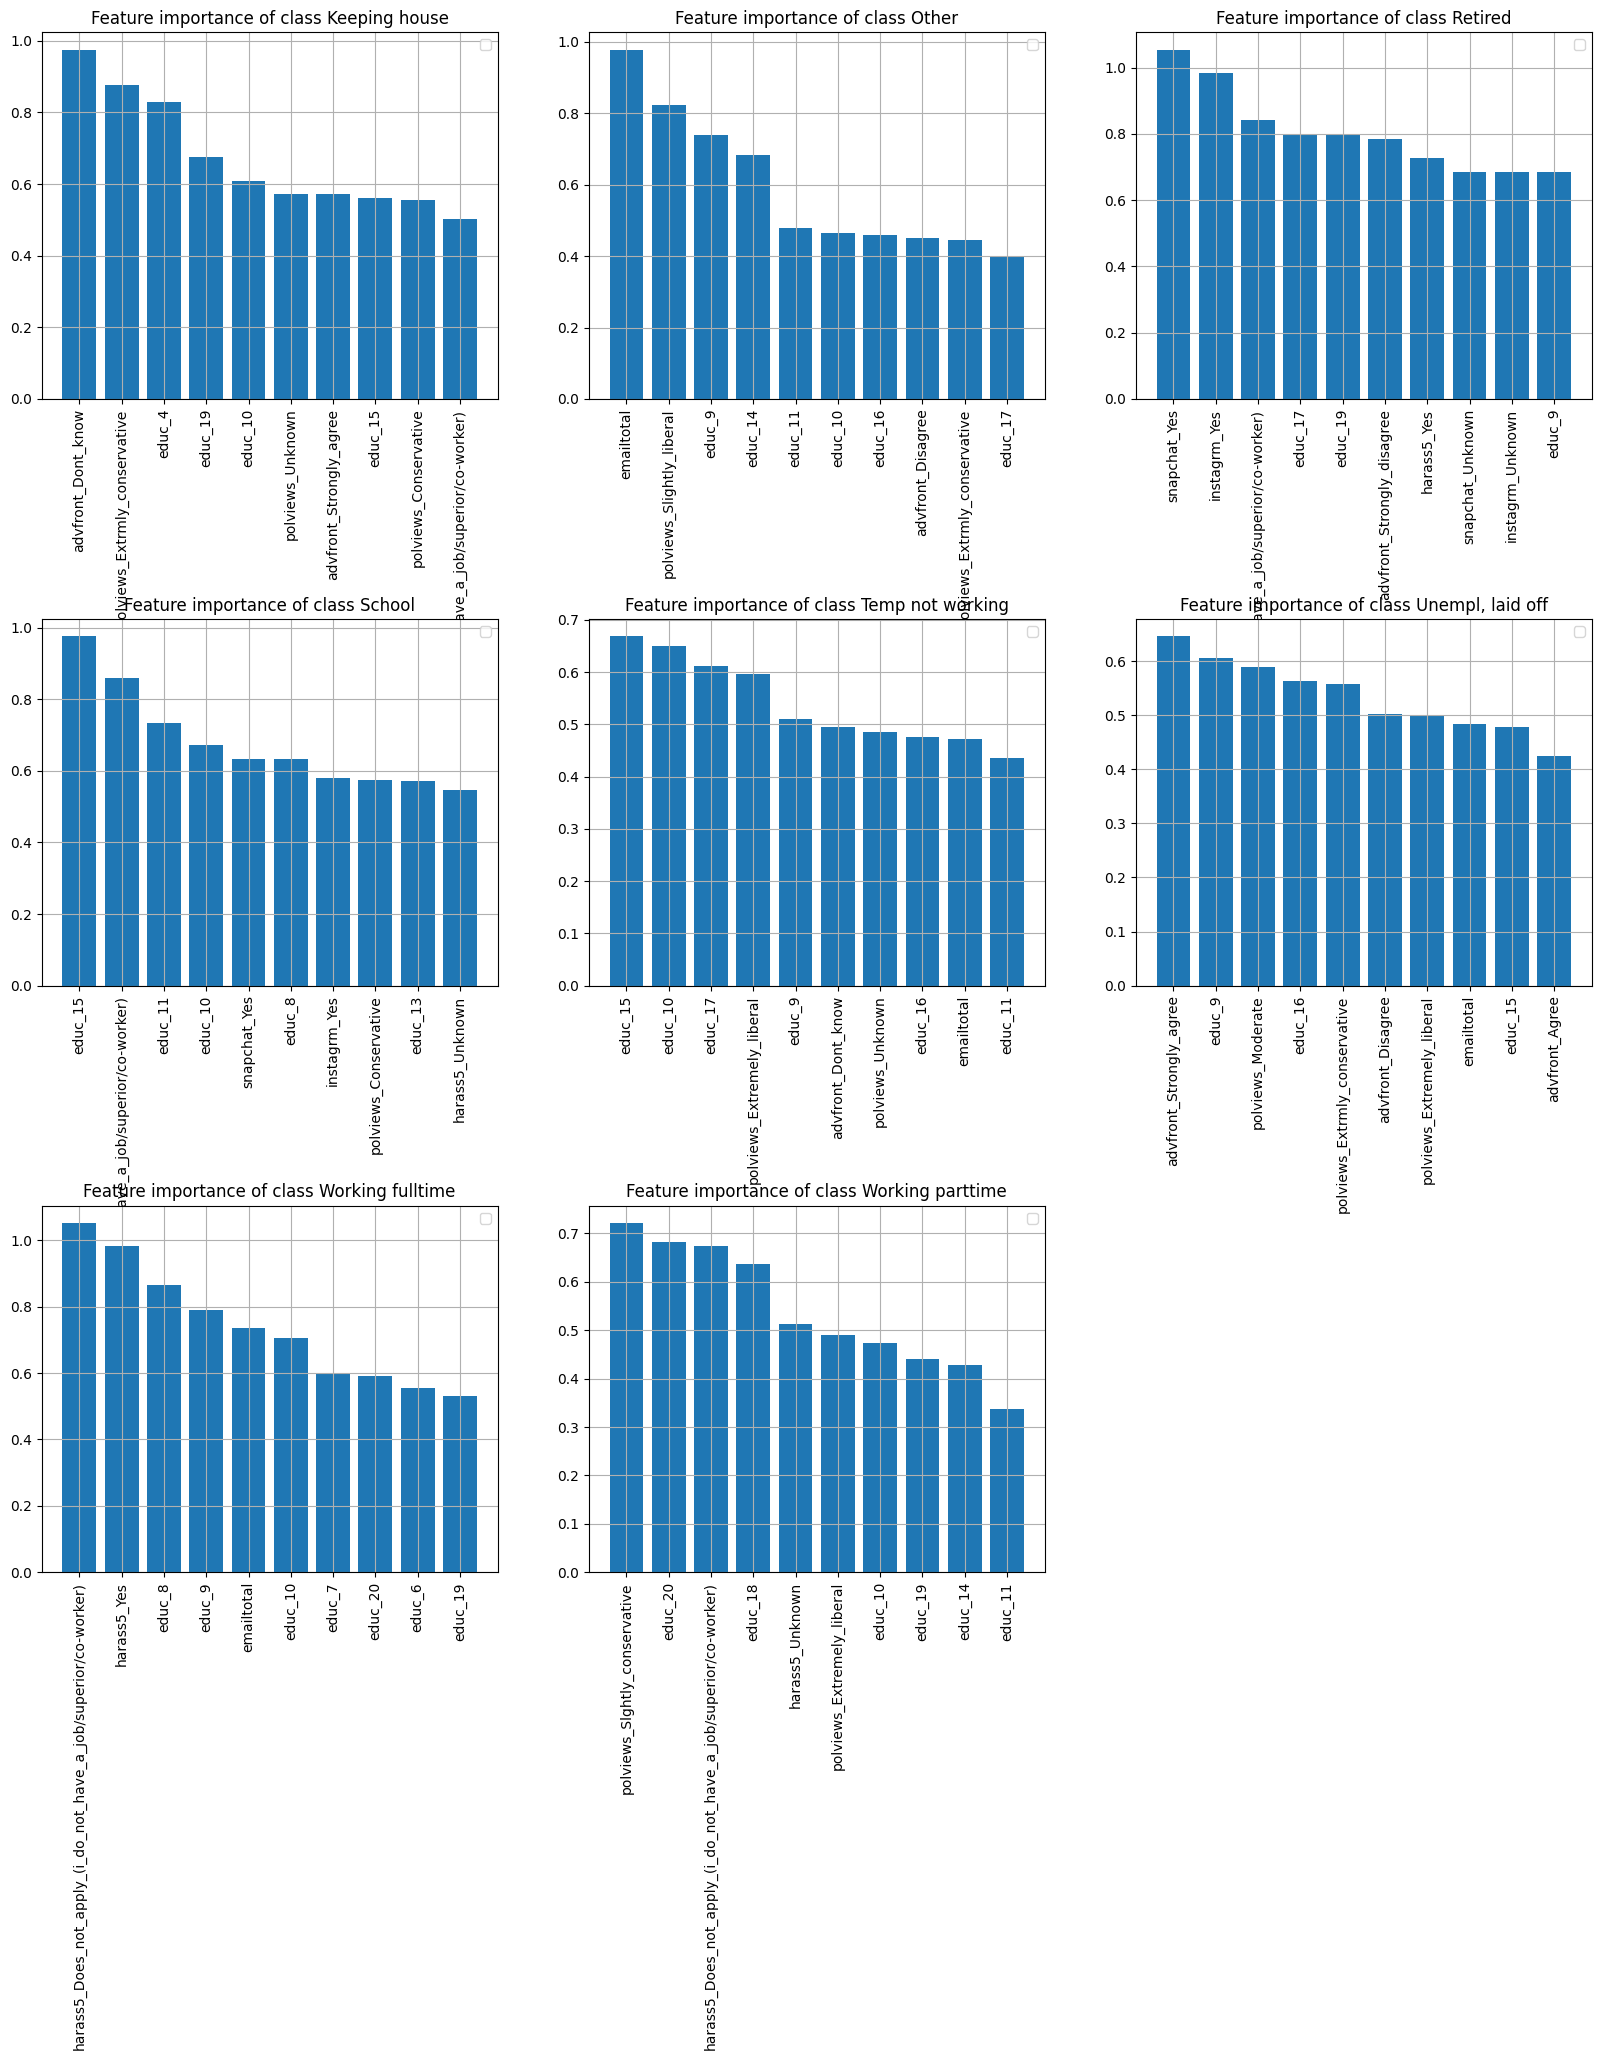
\includegraphics[width=0.6\textwidth]{figures/Thanh/Models/Logistic/Non_null_models_Feature_Importance_Logistic_original_features.png}
        \caption{Biểu đồ cột sắp xếp độ lớn giảm dần (trị tuyệt đối) tham số của các đặc trưng ứng với từng nhãn giả (mô hình với vector đầu vào là vector gốc ban đầu)}
        \label{fig:Non_null_models_Feature_Importance_Logistic_original_features}
    \end{figure}

    Ta có biểu đồ cột sắp xếp độ lớn giảm dần (trị tuyệt đối) tham số của các đặc trưng ứng với từng nhãn giả thể hiện ở hình \ref{fig:Non_null_models_Feature_Importance_Logistic_original_features}.
    Ta nhận thấy các đặc trưng có trọng số lớn tương ứng với từng lớp là educ\_15, snapchat\_Yes, harass5\_Does\_not\_apply đa số là các đặc trưng ít xuất hiện trong tập dữ liệu.

    \begin{figure}[H]
        \centering
        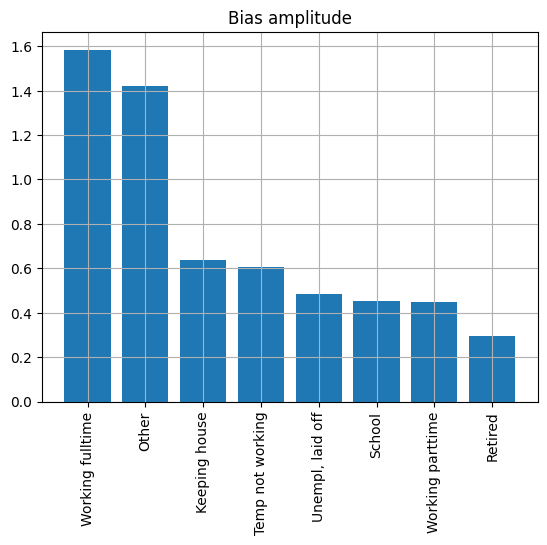
\includegraphics[width=0.6\textwidth]{figures/Thanh/Models/Logistic/Non_null_models_Bias_Importance_Logistic_original_features.png}
        \caption{Biểu đồ cột thể hiện độ lớn của các bias tương ứng với từng nhãn giả (mô hình với vector đầu vào là vector gốc ban đầu)}
        \label{fig:Non_null_models_Bias_Importance_Logistic_original_features.png}
    \end{figure}

    Hình \ref{fig:Non_null_models_Bias_Importance_Logistic_original_features.png} thể hiện độ lớn của các bias tương ứng với từng nhãn.
    Bias tương ứng với nhãn làm việc toàn thời gian có giá trị lớn nhất lý do là vì mô hình có xu hướng phân loại đa số các quan sát vào nhãn làm việc toàn thời gian
\end{enumerate}